\documentclass[paper=a4, fontsize=11pt]{article}
\usepackage[T1]{fontenc}
\usepackage{fourier}

\usepackage[english]{babel}															% English language/hyphenation
\usepackage[protrusion=true,expansion=true]{microtype}	
\usepackage{amsmath,amsfonts,amsthm} % Math packages
\usepackage[pdftex]{graphicx}	
\usepackage{url}

\usepackage[latin1]{inputenc}
\usepackage{graphicx}
\usepackage{times}
\usepackage{multirow}
\usepackage[caption=false]{subfig}
\usepackage{amssymb}
\usepackage{amsmath}
\usepackage{fixltx2e}
\usepackage{subdepth}
\usepackage{enumitem}
\usepackage[latin1]{inputenc}
\usepackage{tabularx}
\usepackage{makeidx}
\usepackage{makecell}
\usepackage[ruled,noend]{algorithm2e}
\usepackage{soul}
\usepackage{array}
\usepackage{xcolor}
\usepackage{amssymb}
\usepackage[figuresright]{rotating}

\newcommand{\red}[1]{{\color[rgb]{1.0,0.0,0.0}{#1}}}
\newcommand{\blue}[1]{{\color[rgb]{0.0,0.0,1.0}{#1}}}

%%% Custom sectioning
%\usepackage{sectsty}
%\allsectionsfont{\centering \normalfont\scshape}

%\usepackage{chngcntr}
%\counterwithout{figure}{section}

%%% Custom headers/footers (fancyhdr package)
%\usepackage{fancyhdr}
%\pagestyle{fancyplain}
%\fancyhead{}											% No page header
%\fancyfoot[L]{}											% Empty 
%\fancyfoot[C]{}											% Empty
%\fancyfoot[R]{\thepage}									% Pagenumbering
%\renewcommand{\headrulewidth}{0pt}			% Remove header underlines
%\renewcommand{\footrulewidth}{0pt}				% Remove footer underlines
\setlength{\headheight}{13.6pt}
\setlength{\textwidth}{15cm}
\setlength{\oddsidemargin}{0.8cm}


%%% Equation and float numbering
%\numberwithin{equation}{section}		% Equationnumbering: section.eq#
%\numberwithin{figure}{section}			% Figurenumbering: section.fig#
%\numberwithin{table}{section}				% Tablenumbering: section.tab#

\def\wrt{w.\,r.\,t.}
\def\eg{e.\,g.}
\def\ie{i.\,e.}
\def\Ie{I.\,e.}
\def\msh{\mathcal{M}}
\def\mds{\mathcal{N}}

\def\pos{\mathbf{q}}
\def\vel{\mathbf{\dot{q}}}
\def\acc{\mathbf{\ddot{q}}}
\def\disp{\mathbf{u}}
\def\mass{\mathbf{M}}
\def\damp{\mathbf{B}}
\def\stiff{\mathbf{K}}
\def\fext{\mathbf{f}_{\text{ext}}}
\def\fint{\mathbf{f}_{\text{int}}}
\def\fcs{\mathbf{f}}

\def\initg{\tilde\Gamma}

%%% Begin document
\begin{document}
	
\begin{center}
\bf{\LARGE Intra-Operative Model-Based Navigation\\ as a Stochastic Filtering}
\end{center}

\section{Introduction}
We use a virtual model of a real object to make \emph{spatial and temporal predictions} about a state 
of the real object being manipulated in a procedure (such as surgical intervention). 
The procedure is \emph{observed} via some modality as a camera, ultrasound, intra-op CT, MRI, 
however, the observation provides only 
\emph{partial and noised information} about the actual state of the real object.
Therefore, the virtual model is employed as a predictive tool in a computer simulation which is running in parallel to the real procedure manipulating the real object.
Nonetheless, since we are in a patient-specific scenario, the virtual model also suffers from uncertainties 
related to some aspects of the model: parameters, boundary and initial conditions. 

This problem can be straightforwardly described as a \emph{stochastic process} which provides a mathematical 
formalization of the model and observations, as well as the uncertainties related to both of them. 
Namely, we are interested in \emph{discrete-time controlled stochastic process}~\cite{grewalkalman}:
\begin{itemize}
	\item Discrete-time: the model of the object, in our case a deformable tissue, is running on a digital computer thus requiring the temporal discretization of the originally continuous formulation given by the theory of elasticity.
	\item Controlled: the model is driven by an external control (here represented by a tool interacting with the tissue).
	\item Stochastic: the model contains uncertainties given by the patient-specific scenario. 
\end{itemize}
In the following, we first introduce the general notion of a non-linear stochastic process. Second, we describe the actual model used for prediction and finally, we show how the problem can be described as a data-assimilation problem. 

\section{General Stochastic Process and Data Assimilation}
\label{s:formal}
In general, a \emph{non-linear discrete-time controlled stochastic process} is formalized as follows:
\begin{eqnarray}
x_k &=& A_{k|k-1}(x_{k-1}, u_{k}, w_{k}) \label{eq:model} \\
z_k &=& H_k(x_k, v_k) \label{eq:meas}
\end{eqnarray}
where
\begin{itemize}
	\item $x_k\in\mathbb{R}^n$ is the state vector,
	\item $z_k\in\mathbb{R}^m$ is the measurement vector,
	\item $u_k\in\mathbb{R}^l$ is the control input vector,
	\item $w_k$ is the \emph{process} noise with co-variance $Q$: $p(w)\sim\mathcal{N}(0,Q)$,
    \item $v_k$ is the \emph{measurement} noise with co-variance $R$: $p(v)\sim\mathcal{N}(0,R)$,
    \item $A_{k|k-1}$ is a non-linear \emph{model transition function} which relates the state $x_{k-1}$ to the next state $x_k$,
    \item $H_k$ is a non-linear \emph{measurement function} which relates the state $x_k$ to the measurement $z_k$.
\end{itemize}
In the classical filtering problem, the system state $x_k$ is estimated given uncertainties related to 
the model ($w_k$), the measurement ($v_k$) and initial condition (or configuration) $x_{k=0}$ where 
it is supposed 
\begin{equation}
x_{k=0} = x_0 + \zeta^x 
\label{eq:initUncent}
\end{equation} 
where $x_0$ is a given initial estimation of the system state and $\zeta^x$ is 
an unknown quantity to be estimated. 

In the data-assimilation scenario, the model uncertainty is intrinsically related to parameters of the model, 
\ie, the model depends on parameters which are known only \emph{approximately}: these can be for example 
the patient-specific biomechanical coefficients, boundary conditions, pre-stress etc. 
Thus, similarly as in~\cite{moireau2011reduced}, we restrict the model uncertainties to the \emph{parameter uncertainties}
globally collected in a vector $\theta\in\mathbb{R}^p$. The aim of the assimilation 
is to estimate both the state vector $x_k$ \emph{and} the the parametric correction $\zeta^\theta$:
\begin{equation}
\theta_k = \theta_0 + \zeta^\theta
\label{eq:param}
\end{equation}
where $\theta_0$ is an \emph{initial estimation} of the parameters. 

Therefore, similarly as in~\cite{moireau2011reduced,wu2007application}, we use the \emph{augmented state vector} $x^a_k$:
\begin{eqnarray}
x^a_{k+1} &=& \displaystyle\binom{x_{k+1}}{\theta_{k+1}}  = \displaystyle\binom{A_{k+1|k}(x_k,\theta_k)}{\theta_{k}} \\
x^a_{k=0} &=& x_0^a + \zeta^a = \displaystyle\binom{x_0 + \zeta^x}{\theta_0 + \zeta^\theta}.
\label{eq:aug}
\end{eqnarray}

% in our case, the biomechanical model of the tissue. 
% The non-linearity is introduced either by co-rotational formulation, or by hyper-elastic formulation 
% which contains two sources of non-linearity: \emph{geometric non-linearity} due to the full Green strain tensor,
% and \emph{physical non-linearity} given by the governing equation, \ie~the stress-strain relationship.

\section{From Deterministic to Stochastic Modeling}
The intra-operative registration scenario is formalized using the apparatus introduced in the previous 
section. First, we put the quantities related of stochastic processes and data assimilation into the context
of intra-operative model-based registration. 

\subsection{Model}
\label{ss:model}
The real object (such as the liver) is modeled using either co-rotational or hyper-elastic
finite element formulation. The problem is defined over a mesh $\msh$ composed of nodes; their actual 
positions and velocities are denoted $\pos$ and $\vel$, respectively. The model is given by motion equation
\begin{equation}
\mass\acc = \fint(\pos,\vel) + \fext
\end{equation}
where $\mass$ is the mass matrix, $\fint$ are the internal forces of the object which depend on 
the nodal positions and velocities and $\fext$ gathers the external forces. 
Using the second-order implicit Euler method, the state $\pos_k$ is obtained as:
\begin{equation}
\pos_k = \pos_{k-1} + h\vel_{k-1} + h^2\acc_{k}
\label{eq:integ}
\end{equation}
where $h$ is the time step and the acceleration $\acc_k$ is obtained by solving the linearized problem
\begin{equation}
(\frac{1}{h}\mass + \damp + h\stiff)\acc_k = \fext - \fint(\pos_{k-1},\vel_{k-1}) - hK\vel_{k-1}
\label{eq:accel}
\end{equation}
where $\damp = \frac{\partial \fint}{\partial\pos}$ and $\stiff = \frac{\partial \fint}{\partial\vel}$
are damping and stiffness matrices. The stiffness matrix contains the material law which determines the 
elastic behavior and response of the tissue. It depends on material parameters such as the \emph{Young's modulus}, 
\emph{Poisson's ratio} in the case of the linear isotropic elasticity. 
Damping matrix is usually approximated using the mass and stiffness matrices.

It remains to specify two aspects of the model described above: first, the vector $\fext$ in 
Eq.~\ref{eq:accel} gathers the \emph{external forces} which are applied to the model as the 
\emph{control inputs}. These can be both the volume forces (such as the gravity) or surface tractions. 

Second, although given a non-zero mass $\mass$, the left-hand side matrix $(\frac{1}{h}\mass + \damp + h\stiff)$ 
is regular, it is often necessary to impose the \emph{boundary conditions}. Here, we consider 
only two types of Dirichlet boundary conditions (DBC). Denoting $\Omega$ the domain of the volume mesh and $\Gamma = \partial\Omega$ 
its boundary (\ie~the surface), we define
\begin{description}
	\item[Homogeneous DBC:] $q^i_k = 0$ for $i\in\Gamma_F$ where $\Gamma_F\subset\Gamma$ is 
	the fraction of surface which is fixed, \ie, the nodes do not move during the simulation
	\item[Heterogeneous DBC:] $q^j_k = p^j_k$ for $j\in\Gamma_P$ where $\Gamma_P\subset\Gamma$ and 
	$\Gamma_P \cap \Gamma_F = \emptyset$ and $p^j_k$ are \emph{prescribed positions}.
\end{description}
The heterogeneous DBC represent another control input of the model, as they are used to displace a surface 
area during the simulation. 

Both conditions can be imposed using either the methods of Lagrange multipliers or penalization.
We assume the penalization is employed, so that the difference between the actual position $q^i_k$ and 
the desired position is penalized using penalization coefficients, \ie, $\kappa(q^i_k - q^i_0)$ for the homogeneous
DBC and $\kappa(q^j_k - p^j_k)$ for the heterogeneous DBC. In the usual scenario where both $\Gamma_F$ and $\Gamma_P$ are known 
\emph{a priori}, the penalization coefficients are usually equal to a positive constant $c$ which is chosen so that 
it is sufficient to impose the condition without jeopardizing the numerical stability of the model.  

\subsection{Stochastic Model: State, Transition Function and Uncertainties}
\label{ss:smodel}
In what follows, we reformulate the quantities introduced in section~\ref{ss:model} in terms of stochastic processes. 

First, in a broad sense, the {\bf state vector} $x$ from Eq.~\ref{eq:model} contains 
both the nodal positions $\pos$ and velocities $\vel$. 
In case we assume that the object is not moving initially, thus $\vel_{k=0} = \mathbf{0}$,  
the initial velocity uncertainty $\zeta^\vel$ (c.f. Eq.~\ref{eq:initUncent}) is zero.
Consequently, only the position $\pos$ is included in the state vector.

Further, the integration scheme given by Eq.~\ref{eq:integ} and~\ref{eq:accel} yields the 
{\bf transition function} A in Eq.~\ref{eq:model}: given $\pos_{k-1}$ (and $\vel_{k-1}$),
it computes the actual state $\pos_k$. The problematic of measurement and observation (Eq.~\ref{eq:meas}) is postponed to section~\ref{ss:obser}. 

As we are interested in data assimilation, we consider the 
augmented version given by Eq.~\ref{eq:aug}. Then, the vector $\theta$ consists of {\bf model parameters}: 
these can be represented either by the biomechanical coefficients such as the 
Young's modulus. Nevertheless, the augmented scheme also allows for an estimation of boundary conditions.
In the following, we focus on the former where we suppose that the domain $\Gamma_F$ is not 
known exactly (\eg, due to the occlusion). 

As introduced in section~\ref{ss:model}, the nodes with prescribed homogeneous Dirichlet conditions 
are associated with non-zero penalty coefficient $\kappa=c$. 
Without loss of generality, this definition of homogeneous Dirichlet conditions can be reformulated 
as follows: for all nodes $i\in\Gamma$, a penalty factor $\lambda^i$ is defined so that 
$\forall i\in\Gamma_F: \lambda^i = 1$ and $\forall j\in\Gamma\setminus\Gamma_F: \lambda^j = 0$.
The penalty coefficients are then computed as $\kappa=\lambda^ic$; for free nodes $\kappa = 0$, thus 
no homogeneous boundary condition is imposed.

The estimation of the unknown homogeneous boundary conditions is now equivalent to estimating the values $\lambda^i$. 
For this purpose, we introduce a set $\initg\subset\Gamma$, an initial area 
for which the penalty factors $\lambda^i$ are to be estimated: it can be chosen for example as $\initg=\Gamma\setminus \Gamma_P$, 
or it can be constructed according to some \emph{a priori} information, \eg, it may contain nodes which 
are close to anatomical landmarks such as ligaments. The estimation should result in a decomposition
$\initg = \tilde\Gamma_0\uplus\tilde\Gamma_1$ s.t.
\begin{itemize} 
	\item $\forall i\in\tilde\Gamma_1: \lambda^i\rightarrow 1$, \ie, the nodes in $\tilde\Gamma_1$ are fixed, so 
	$\tilde\Gamma_1$ converges to $\Gamma_F$,
	\item $\forall j\in\tilde\Gamma_0: \lambda^j\rightarrow 0$, \ie, the nodes in $\tilde\Gamma_0$ are free, thus
	not influencing the simulation.  
\end{itemize}
In other words, the estimation of boundary conditions is reformulated as an estimation of a parameters
$\zeta^\lambda$ such that $\lambda = \lambda_0 + \zeta^\lambda$ is a penalty factor and $\lambda_0$ is  
its initial value. This is equivalent to Eq.~\ref{eq:param} and thus $\lambda$ is included in the augmented 
stochastic state. 


\subsection{Observations and Measurements}
\label{ss:obser}
The stochastic process requires \emph{observation}, a comparison of the actual estimated state \wrt~the 
state of the real object. However, the latter is typically not available completely, but only via noised and/or partial 
measurement. In general, the observation is formally represented by the non-linear operator $h$
in Eq.~\ref{eq:meas}. 

{\bf Observability.} 
In~\cite{grewalkalman}, notion of \emph{observability} is introduced, but only for a linear time-invariant systems:
assuming $\mathbf{A}$ the transition function of a \emph{linear} dynamic system and $\mathbf{H}$ 
the \emph{linear} observation operator, then observability can be characterized by the rank of matrices 
\begin{equation}
[ \mathbf{H}^{\top} \qquad \mathbf{A}^\top\mathbf{H}^{\top}  \qquad (\mathbf{A}^\top)^2\mathbf{H}^{\top}  \qquad \cdots  \qquad (\mathbf{A}^\top)^{k-1}\mathbf{H}^{\top} ]
\end{equation}
\blue{I think this should be the key aspect of out work, since it should provide 
us with a tool capable of address quantitatively the following issues: 
\emph{What is the minimal information provided by the observation such that it allows for prediction with required accuracy?} 
I have to look at this problematics more closely; this is only the first attempt to come up with a formal framework. 
At the same time, I am quite sure that this framework is quite powerful and allows for precise formulation of the problem, 
which in turn leads to a solution such as the corresponding filter.
A very naive visualization of our preliminary reflections is given by Fig.~\ref{f:scheme}.}

\begin{figure}
	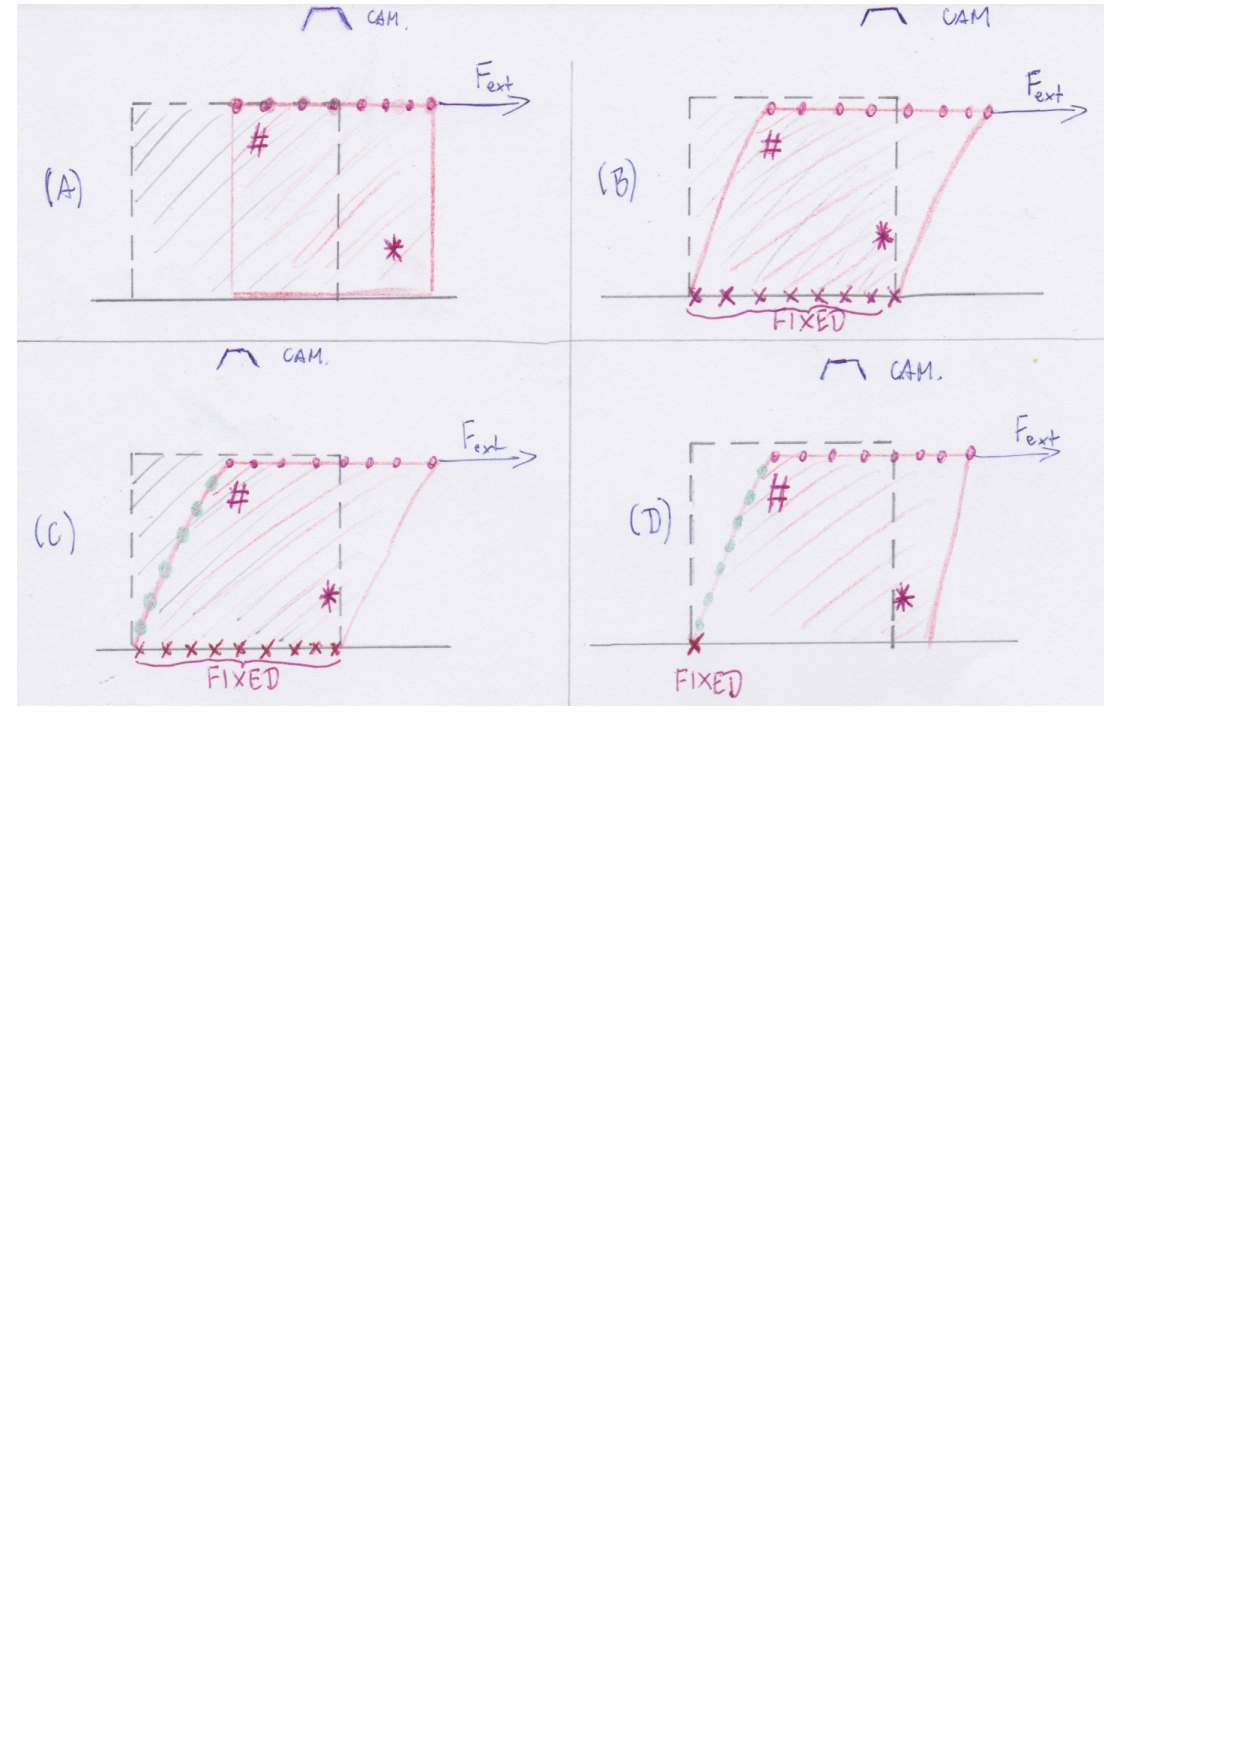
\includegraphics[width=\textwidth]{figs/schemeObservations.pdf}
	\caption{Four different scenarios where the position of a features (red * and \#) are to be predicted. If we suppose a naive approach where only the points on the upper face (red bullets) are being tracked, already the difference between (a) and (b) is unobservable. If we add more points (green bullets), the two difference between (a) and (c) becomes observable, however: (i) these points must be added during the procedure: how to find the correspondences reliably? (this shows that the observation operator must be revisited quite a lot) and (ii) anyway, the difference between (c) and (d) remains unobservable and IMHO it cannot be distinguished without additional information (given by some other modality than the camera placed at the top). 		
		Moreover, the above (un-)observability plays a crucial role in the prediction of the * position. The position of \# feature is quite well predicted in all cases, thus the sensitivity of prediction error \wrt~given scenarios is different for each feature.  
	    Therefore, I think that the observability should take into account the position of the feature that is to be predicted. 		
		}		
	\label{f:scheme}
\end{figure}




\bibliographystyle{unsrt}

\bibliography{biblio}


\end{document}
